 
\chapter{AP models of atrial cells}
\label{chap:ap-models-atrial}

\section{Introduction}

Atrial cells are pacemaker of the heart. Early cardiac cellular models targetted
to atrial cells, Fig.\ref{fig:SA_AP}.

\begin{figure}[hbt]
  \centerline{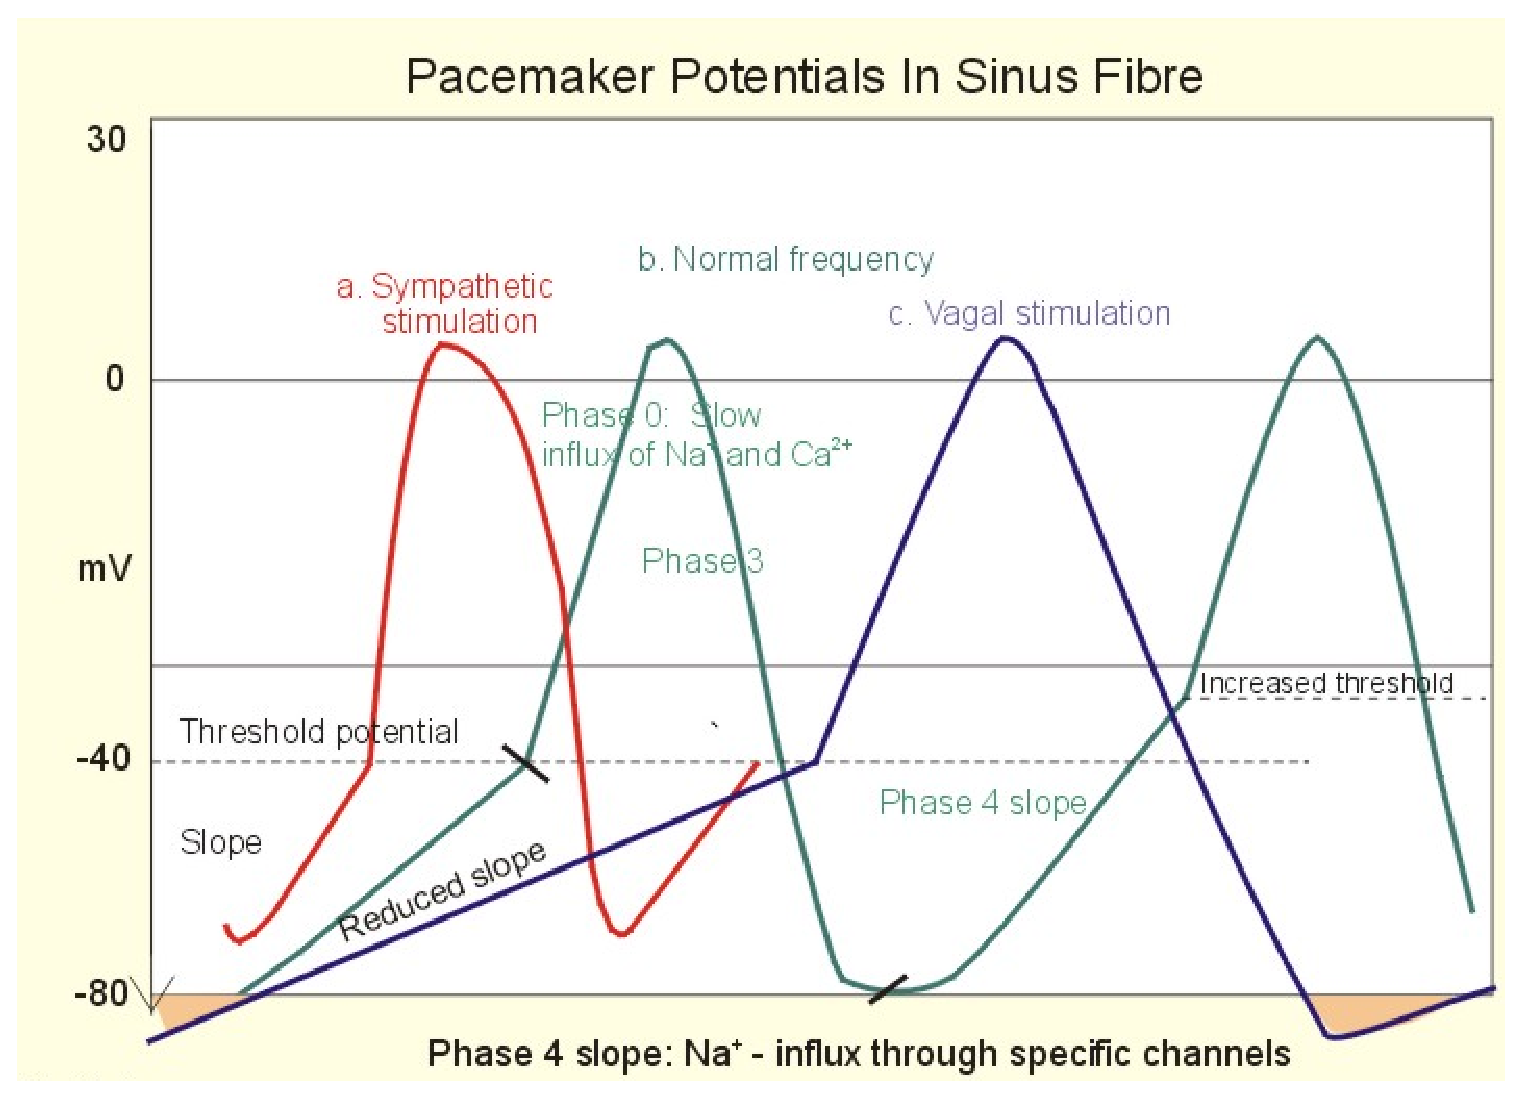
\includegraphics[height=5cm,
    angle=0]{./images/SA_AP.eps}}
  \caption{Pacemaker activities under (a) sympathetic stimulation; (b) normal;
  (c) vagal stimulation}
\label{fig:SA_AP}
\end{figure}

Like ventricular myocytes, CICR is the meachanism of releasing calcium during
EC-coupling of atrial cells. However, the rise of calcium starts initially at
the cell surface and then propagates as a wave of CICR into the cell interior
\citep{huser1996, mackenzie2001, tanaami2005}. In ventricular myocytes, removing
the T-tubule systems result into the similar spatiotemporal properties of atrial
cells \citep{brette2002}. This studied shown that the fundamental differences
between atrial cells vs. ventricular myocytes is the lack of T-tubules in atrial
cells. So, the RyR see the calcium in the myoplasm rather than the calcium in
the subspace. 

Compared to ventricular myocytes, there are also difference in expression levels
of different proteins, e.g.
\begin{enumerate}
  \item NCX: in human atrium, NCX protein levels are 50\% as seen in ventricle
  \citep{wang1996}
  \item SERCA: in rat and mouse, Phospholamban (PLB) is expressed less
  strongly in the atrium, giving PLB:SERCA2a ratio 4-5 times
  less in the atria than in ventricle \citep{koss1997, freestone2000}.
  This means SERCA2 activity is higher, or sequestering $\Ca$ back
  to SR faster, enhancing the rate of relaxation in atrium (or shorter APD in
  atrium).

  SR $[\Ca]_\SR$ content is  
  and $[\Ca]_\myo$ at rest is 
  
    
  \item IP3R: greater expression in atrium, and localises close to the RyR
  which potentially alters ECC with arrhythmogenic $\Ca$ release
  during diastole \citep{lipp2000, mackenzie2002}
  
  \item Intracellular buffer: buffering power is substantially greater in the
  atria
  
  \item The capacitance to volume factor is 14.6 pF/pL in atrial cells
  \citep{walden2009} vs. 6.76 pF/pL in ventricular myocytes \citep{satoh1996svr}.
\end{enumerate}
Overall, there is a marked differences in the amplitude and kinetics of systolic
$\Ca$ transients, in rats \citep{walden2009}.
In cardiac cells, less than 1\% of calcium released is free in the cytosol; the
remainder is bound to various intracellular $\Ca$ buffers \citep{berlin1994iccb,
trafford1999nrr}; with the major 'fast' buffers are SERCA and Troponin-C. 
  

No difference in diastolic $[\Ca]_\myo$ was found between atrial and ventricular
myocytes. So, using $[\Ca]_{i,\rest}=0.9xx \muM$ is okay in rat atrial cells.
However, the amplitude of systolic $\Ca$ transient is 34\% smaller in atrial
(i.e. 0.251$\muM$ in atrial cells vs. 0.376$\muM$).

\section{Moe-Rheinboldt-Abildskov (1964)}

The classical concept of atrial fibrillation (AF) was first formulated with
wavelet hypothesis where a cluster of cells when firing generate a wavelet (a
small wave), and when the number of wavelets triggered at the same times are big
and closed enough to each other, it can trigger the full wave. It was tested
with a simple cellular-automaton computer model \citep{moe1964}, where each
cell interacts with 6 neighbors.

\section{Hilgemann-Noble model 1987 (rabbit multi-cell)}
\label{sec:hilg-noble-model}

Based on DiFrancesco-Noble model for Purkinje fiber
(Sect.~\ref{sec:difr-noble-purk}),~\citep{hilgemann1987} developed a model for
the rabbit atrial cell.  This is multicellular model as the data is based on a
'preparation' of multiple cells. It doesn't aim to reproduce single cell
behavior; but an overal behavior at tissue level. That's why all the data
measured is very large. Mechanism for calcium-induced calcium release (CICR) has
been taken intou account; yet the formulaism was not mechanistically correct.

\begin{framed}
  Components essential to EC coupling are: (1) sodium channel, (2)
  electrogenic SERCA pump, (3) background sodium and calcium
  conductances, (4) calcium channel, (5) electrogenic sodium-calcium
  exchange mechanism, and (6) instantaneous potassium
  conductances. 
\end{framed}

At the tissue level, \textcolor{red}{the model also simulated the transient of
extracellular calcium}, previously presented in abstract form in
\citep{hilgemann1986}. Giving the total ''preparation'' volume as 1.6nL with
total 60 cells in the preparation, 40\% are extracellular space, and another
40\$ for cytoplasmic volume. As this cytoplasmic volume underestimate the volume
of mitochondria and nuclei; they decided to reduce the cytoplasmic volume to
25\%, i.e. giving identical effect of decreasing cytosolic buffers capacity by
30\%.

\begin{framed}
Assuming an atrial cell as a cylinder with an average diameter of 5-6 $\mu$m and
an average cell length of 125 $\mu$m, the average cat atrial cell volume would
be 15 pL. 
\end{framed}

A total capacitance of 6 nF was used for the simulations (or 0.1 nF per cell
given that there are 60 cells in the preparation); this is twice the capacitance
expected if the cells were simple cylinders with volume 15pL, and specific
capacitance $\Csc = 1 \mu$F/cm$^{-2}$. This reflects the possibility that atrial
cells may have substantial membrane invaginations and/or T-tubules.

\subsection{Hypothesis analysis}

\begin{enumerate}
  \item {\bf fast $\Na$ current}: like \citep{difrancesco1985mcea}, the
  conductance was selected to give the peak of membrane potential is achieved after 1.5ms
  after passing the threshold -55 mV; giving net increase $\Delta [\Na]_i =
  4.2\muM$ per action potential or total $\Na$ influx is 2.5$\mu$mol/(kg fresh
  mass).
  \item {\bf $\Na$ pump}: like \citep{difrancesco1985mcea}, maximum pump rate
  was 6 mmol/(kg fresh mass)/min to give proper $\Na$ homeostasis
  
  \item {\bf background $I_\bCa, I_\bNa$}: the background $I_\bNa$ was selected
  to bring resting $[\Na]_i=3.5$mM (with the pump rate selected above); and
  $I_\bCa$ was selected to bring $[\Na]_i$ to 5mM via the NCX. The initial resting
  $[\Na]_i=7$mM which correspond to the steady-state value reaching with 0.5Hz
  stimulation.  
  
  \item {\bf PMCA pump}: The sarcolemma calcium pump (PMCA) was modeled in some
  simulation both with and without electrogenicity. Like
  \citep{difrancesco1985mcea}, it was treated as an optional calcium extrusion
  mechanism without electrogenicity. It is being modeled as rate proportional to
  instataneous $\Ca$ binding to a single binding site with dissociation constant
  $K_{d,\PMCA}=0.0002$mM.
  \begin{equation}
    \label{eq:1418}
    J_\pmca = k_\pmca \frac{[\Ca]_i}{[\Ca]_i+K_{d,\PMCA}}
  \end{equation}
  

  \item {\bf NCX}: the major calcium extrusion mechanism in almost all
  simulation. The stoichiometry Na:Ca=3:1 is assumed.

  
%   \item {\bf background $I_{b,\Na}$}: like \citep{difrancesco1985mcea}

  
  \item {\bf $\K$ conductances} and {\bf inward rectifier}: To study the
  isolated effect of NCX and LCC only, the time- and calcium-dependent outward
  current has been avoided and this current was treated as instantaneous using
  linear conductance, with magnitude set large enough to give AP of realistic
  duration, i.e. membrane potential repolarization at the speed found in
  experiments in the positive range to mid-voltage range. The inward rectifier
  was set large enough to terminate the AP at a realistic rate.
  Thus, the inward rectifier was shifted 30mV to more positive potential from
  the value used in \citep{difrancesco1985mcea}.
  
  As in rabbit atrium, the transient outward $\K$ current with a
  characteristics of an 'A-current' and a linear background conductance play an
  important role, the current has been added for two simulations, using the
  formula, with steady-state activation
  \begin{equation}
  \label{eq:hilgemann1987_34}
  f_{ss} = \frac{1}{1+\exp\left( -1/5(E_m+4) \right)}
  \end{equation}
  and inactivation was assumed negligible. The fractional activation of $I_\to$
  conductance $f_{act}$ was simulated using
  \begin{equation}
  \label{eq:hilgemann1987_35}
  \frac{df_{act}}{dt} = 333.(f_{ss}-f_{act})
  \end{equation}
  and the linear background potassium conductance was responsible for terminal
  repolarization. 
% \item $I_\ca$ conductance: like \citep{difrancesco1985mcea}


\item {\bf Delayed $\K$ current}: The role of time-dependent (delayed) $\K$
current was assumed to be negligble in action potential in the simulation of the
study. The role of time-dependent (delayed) change in K+ conductance is, in any
case, thought to be very small in action potentials of the kind simulated here.

% \item Time- and calcium-dependent $\K$ conductances were not generally
% simulated in order to study the isolated influences of calcium
% channels and sodium-calcium exchange on action-potential
% configuration. 
 
  \item {\bf SERCA pumps}: different strategies were tested, starting from
  simple to more complicated formulation
  \begin{enumerate}
    \item calcium uptake and loss from the SR is formualted as linear rate
    \citep{difrancesco1985mcea}
    \item calcium uptake is proportional to calcium binding to a single site,
    with a translocation process, i.e. 4-step ATPase cycle as  in
    Fig.~\ref{fig:Hilgemann_Ca} which allows the enzyme to operate in  2 mode
    (forward\footnote{pump $\Ca$ into SR} and reverse\footnote{release $\Ca$
    from SR to cytosol}). 
    
    \item calcium uptake is proportional to calcium binding to two sites with
    cooperativity, with a translocation process, i.e. 6-step ATPase cycle
    \citep{inesi1980} (Sect.\ref{sec:inesi-et-al}).
  \end{enumerate}
  The second approach was being used in the model. The $\Ca$ binding and
  translocation of $\Ca$-bound enzyme were treated as instantaneous (denoted by
  single double-arrow line). So, only dissociation constant $K_d$ (e.g.
  $k_{xcs}, k_{srca}, k_{cyca}$) are needed.
  The fraction X of enzyme in the 4 conformations:
  \begin{enumerate}
  \item $[X]_\cy$: fraction of empty enzyme that the $\Ca$ binding
    site face the cytosol. The higher this fraction, the more calcium is uptake.
    
  \item $[X]_\sr$: fraction of empty enzyme that the $\Ca$ binding
    site face the SR. The higher this fraction, the more calcium is being
    released to cytoplasm. 
  \item $[X_c]_\cy$, $[X_c]_\sr$: fraction of calcium-bound enzyme
  \end{enumerate}
The flux in the direction of uptake $\Ca$, and is defined in terms of a change
in cytosolic calcium concentration (i.e. the reference volume is cytosolic
volume) is
  \begin{equation}
    \label{eq:1416}
    J_\serca = \alpha [X_c]_\cy - \beta [X_c]_\sr
  \end{equation}
 $\Ca$ uptake decreases with the increase in SR calcium load. \textcolor{red}{If
 the rate-limiting step a reaction closely related to binding of the first calcium
 iion; then the kinetics of calcium transport here need not be very different
 from models involving two-calcium binding sites}.
  
  \begin{figure}[hbt]
    \centerline{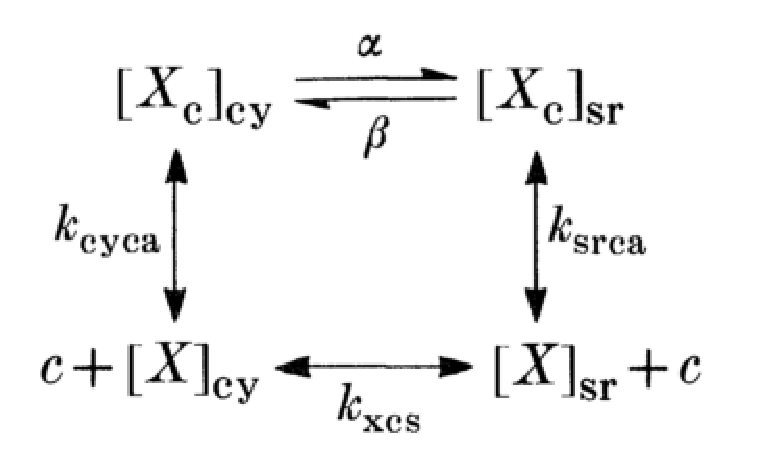
\includegraphics[height=3cm,
      angle=0]{./images/Hilgemann_Ca.eps}}
    \caption{SERCA pump}
    \label{fig:Hilgemann_Ca}
  \end{figure}
  \begin{equation}
    \label{eq:1417}
    \begin{split}
      K_1 &= k_{cyca}k_{xcs}/k_{srca} \\
      K_2 &= [\Ca]_i + [\Ca]_\sr K_1 + k_{cyca}k_{xcs}+k_{cyca}\\
      [X_c]_\cy &= \frac{[\Ca]_i}{K_2} \\
      [X_c]_\sr &= [\Ca]_\sr\frac{K_1}{K_2}\\
      [X]_\cy &= k_{cyca}/K_2 \\
      [X]_\sr &= k_{cyca}k_{xcs}/K_2
    \end{split}
  \end{equation}
  with $k_{cyca}=0.0003$mM, $k_{srca}=0.5$mM, $k_{xcs}=0.4$. $\alpha$
  was chosen high enough to give the desire time course of relaxation
  of $[\Ca]_i$, and $\beta$ was set to keep the reaciton with $K_d=k_{xcs}$. 

NOTE: Using 2 calcium binding sites or sequential binding steps do not
necessarily give a much different kinetics with single calcium binding
site above. 

\item {\bf Cytosolic $\Ca$ buffering}: $\ce{Ca + B <=>[k^+][k^-] CaB}$
  \begin{equation}
    \label{eq:1419}
    \frac{d[\CaB]}{dt} = k^+([\B]_T-[\CaB])[\Ca]_i-k^-[\CaB]
  \end{equation}
  The slow off-rates ($< 50$sec$^{-1}$) would not permit enough loading of SR,
  and giving high $[\Ca]_i$ upon repolarization as as a consequence a large
  portion of calcium is extruded by the NCX. So, off-rates should be high enough
  ($> 150$sec$^{-1}$ which is in the range of isolated Troponin C). So,
  \textcolor{red}{fast buffering was assumed}. 
  
  In the model, two types of buffers are assumed: X1 and X2.
  \begin{enumerate}
  \item X1 (Troponin C + SR pump + membrane binding sites): with
  $K_{m,X1}=2\mu$M (with $k^+=10^2$[1/($\mu$M.s)], $k^-=200$ [1/s]) and
  $[X1]_T=180\mu$M~\citep{robertson1982}. 
    Among the total buffer, $140\mu$M was assumed to be Troponin C
    (i.e. 24$\mu$mol/kg fresh mass);
    the remainder represents other $\Ca$ binding sites with moderately
    high affinity.

  \item X2 (Calmodulin): with off-rate 4 time slower
  than X1 (i.e. $K_{m,X2}=8\mu$M) meaning it binds more calcium at low cytosoic
  calcium concentration, and $[X2]_T=20\mu$M (i.e. 8$\mu$mol/kg fresh mass)
  \end{enumerate}
  So, the total cytosolic buffer was 200$\muM$.
  
\end{enumerate}

New formulations compared to DiFrancesco-Noble model are
\begin{enumerate}
  \item $I_\ca$: A good formulation of calcium current via $\Ca$-channels should
  (1) possess both calcium-dependent and voltage-dependent inactivation
  mechanism, (2) potentially explain extremely prolonged extracellular calcium
  depletion responses found under some experimental settings, as well as
  extremely prolonged calcium currents found in atrial cell with strong internal EGTA loading.
  
  $\Ca$-dependent inactivation play a major role in preventing not only calcium
  overload, but also sodium overload. Here, it's assumed that $\Ca$-dependent
  inactivation is assumed to be followed by $V_m$-dependent inactivation.
  In particular, $\Ca$ inactivates the channel by binding to a regulation site,
  i.e. inactivation state $F_{\ce{CO}}$; this inactivation is preserved (or
  prolonged) by an inherently  $V_m$-dependent inactivation process leading to
  $F_{\ce{CV}}$ which occurs slowly  under the absence of $\Ca$.
  So, totally, there are 4 states:

  \begin{equation}
    \label{eq:1414}
    \begin{split}
      \ce{OO <=>  CO} \\
      &\Updownarrow \;\;\;\;\;\;\;\;\;\;\; \Updownarrow\\
      &\ce{OV <=> CV }
    \end{split}
  \end{equation}
  
  It's assumed that only OO is the conducting state; with fraction of channels
  is $F_{OO}$. NOTE:
  \textcolor{blue}{Some may want to treat OV or CO with partial conducting
  states; yet it's not examined here}. $F_C=F_{CO}+F_{CV}$ is the fraction of
  $\Ca$ channels with regulatory site occupied by $\Ca$;
    and $F_V=F_{OV}+F_{CV}$ is the fraction of channel
  inactivated by $V_m$-dependent process.  For simplicity, the binding of $\Ca$
  is assumed instantaneous so that the fraction of channels in calcium-binding
  state can be modelled as linear algebra formula, rather than ODE. The equation
  for $F_V$ is still ODE.
  \begin{equation}
    \label{eq:1415}
    \begin{split}
      F_C &= \frac{[\Ca]_i}{0.001+[\Ca]_i} \\
      \frac{dF_V}{dt} &= \left( F_{OO} + 120 F_{CO} \right) \beta - F_V \alpha
      \\
      \beta &= \frac{2.5}{1+\exp(-\frac{1}{4}(V_m+34))} \\
      \alpha &= 6.25\frac{V_m+34}{\exp(\frac{1}{4}(V_m+34))-1}
    \end{split}
  \end{equation}
\textcolor{red}{This formulation only
  minimize, but not completely eliminate the activation} of $\Ca$ channels
  during relaxation. 
  
 
 \begin{figure}[hbt]
  \centerline{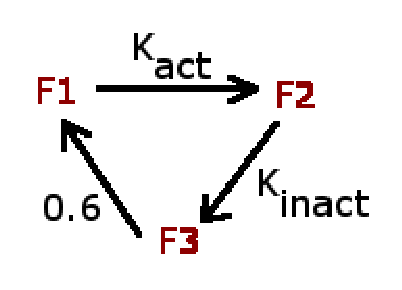
\includegraphics[height=3cm,
    angle=0]{./images/Hilgemann1987_CICR.eps}}
  \caption{Life cycle of the activator $F_2$ from precursor $F_1$, to product
  $F_3$}
\label{fig:Hilgemann1987_CICR}
\end{figure}

 \item CICR was (wrongly) modeled as the instantaneous binding of two activator
 $F_2$ to the release channel, with binding constant $K_{d,F2}=0.25$; giving the
 fraction of open release-channel $F_r$:
 $F_r=\left(\frac{F_2}{F_2+K_{d,F2}}\right)^2$.
 
 The activator $F_2$ is assumed to be produced from the precursor $F_1$,
   and also quickly degrade into product $F_3$, as shown in
   Fig.\ref{fig:Hilgemann1987_CICR}. $F_3$ is generated slowly to the precursor
   $F_1$. They are all given by the ODEs
   \begin{eqnarray}
   \frac{dF_2}{dt}=F_1 K_{act}-F_2K_{inact}\\
   \frac{dF_3}{dt} = F_2 K_{inact} - 0.6 F_3\\
   \frac{dF_1}{dt} = 0.6F_3 - F_1 K_{act}
   \end{eqnarray}
   with $K_{act}=600(E_{on}+R_c)$, and $K_{inact}=100+1000R_c$. Here, $V_m$ initiate the
   activation process from $F_1$ to $F_2$, defined by the function
   $E_{on}=\exp\left(0.08(V_m-40\right)$. Another activation factor $R_c$ is the
   calcium binding at two regulatory calcium binding sites, with an
   arbitrary binding constant $K_d=0.5\muM=0.0005$mM (the value in the range
   0.4-0.5$\muM$ gave the best result for the difference in $V_m$-dependence of
   calcium release). So, $R_c =\left(\frac{[\Ca]_i}{[\Ca]_i+0.0005}\right)^2$.

	Finally, calcium release is defined as
   \begin{equation}
   J_\rel = (F_r K_{\max,\ca}+K_\leak)
   %[\ca]_{rel}.K_{\max,\ca}
   \end{equation}
   with $K_{\max,\ca}$ is the maximal release rate. The effect of an agents
   though to activate the release channel causing a passive calcium leak from
   SR at a constant level was modeled as $K_\leak$ [no value available].
   
   \item SR was modeled with two compartment: an uptake compartment with
   $[\Ca]_{u}$ and release store compartment with $[\Ca]_{rel}$ (which is
   equivalent to network SR and junctional SR in later models). The diffusion of
   calcium from uptake to release store was based on time constant of 20ms. This
   step is treated as instantaneous
   \begin{equation}
   J_\xf = k_{trans}\left([\Ca]_{u} - [\Ca]_{rel}\right)
   \end{equation}
   and 
   \begin{eqnarray}
   \frac{d[\Ca]_{u}}{dt} = -J_\xf + \frac{1}{f_{sr,up}}J_\serca \\
   \frac{d[\Ca]_{rel}}{dt} = 
   \end{eqnarray}
   with fractional volume (w.r.t cytosolic volume) $f_{sr,up}=V_{cyt}/V_{up}$
\end{enumerate}


% For the sake of brevity, extensive citations concerning the individual
% mechanisms simulated will not be given here; the wealth of available
% literature is, however, readily accessible from the major articles
% cited. After performing the original simulations, multiple
% formulations were

\subsection{Mathematical model}

CONVENTION: The units with time are in seconds (sec), and concentration are
in mM (mili mol/L cyto.).

The equation
\begin{equation}
\frac{d[\Ca]_i}{dt} = J_{I_\ca} + J_\ncx - J_\serca + J_\xf - J_\pmca
\end{equation}

Extracellular calcium was treated as an ODE, giving time constant of 5min for
calcium equilibrium (i.e. calcium exchange to the muscle bath play no role in
this simulation).
\begin{equation}
\frac{d[\Ca]_o}{dt} = ([\Ca]_b - [\Ca]_o) k_{diff} -
\frac{1}{f_{exsp}}\left(J_{I_\ca} + J_\NCX - J_\pmca\right)
\end{equation}
with $[\Ca]_b$ is the assumed muscle bath calcium concentration; the fractional
volume of the extracellular space in relation to cytosolic volume
$f_{exsp}=V_{ex}/V_{cyt}$ (which is 1.0 in the simulation); the time constant
$k_{diff}$ (set to 0.0).

\subsection{Numerical method}
\label{sec:numerical-analysis-5}

The simulation was performed on Compaq Deskpro and IBM AT personal
computers equipped with the INTEL 80287 mathematics coprocessor, in
the TURBO Pascal language (Borland International, Scotts Valley,
California). The integration method is given in \citep{difrancesco1985mcea}.  

It took 48h, which correspond to 500 excitation cycles. Conservation was
maintained to an accuracy of better than 1\%. The result is the software named
OXSOFT HEART.

\subsection{Analysis}

Calcium current is fully activated after 2ms of excitation, and substantially
inactivated after 30ms.  The total cytosolic calcium increased in the simulation
was 120$\muM$, giving total free calcium concentration gained was 2.6$\muM$.
This magnitude of increase corresponds to 30$\mu$mol calcium/(kg fresh mass)
\citep{fabiato1983cir} or about 50\% of maximum tension developed by cardiac
muscle, but nearly maximal twitch in an intact muscle. 

NCX resist repolarization from approximately -30mV. 

\begin{figure}[hbt]
  \centerline{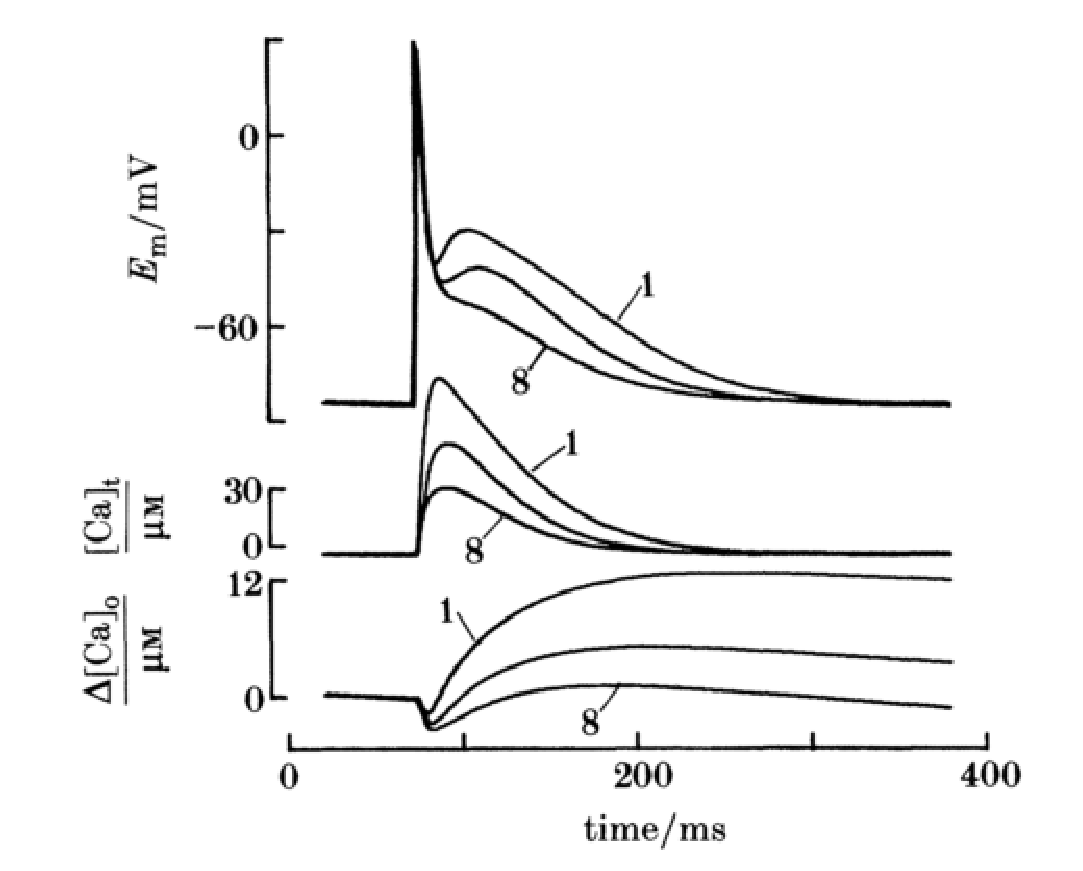
\includegraphics[height=6cm,
    angle=0]{./images/Hilgemann1987_Ca-transient.eps}}
  \caption{Top: AP; Middle: Calcium transient $[\Ca]_i$; Bottom:
  Extracellular calcium transient. Adopted from  \citep{hilgemann1987}}
\label{fig:Hilgemann1987_Ca-transient}
\end{figure}


20 different formulas for CICR were assumed.  A sarcolemmal calcium (SERCA) pump
was treated as an optional mechanism, and sodium-calcium exchange is the sole mechanism of
calcium efflux in all simulations presented except one. 

Large movement of calcium between the extracellular and cytoplasmic region can
take place without any contraction. 

\section[Earm-Noble model (1990)]{Earm-Noble model (rabbit) (1990)}
\label{sec:earm-noble-model}

This is a single-cell model developed based on Hilgermann-Noble multicellular
model~\citep{hilgemann1987} (Sect.\ref{sec:hilg-noble-model}). The purpose is to
replicate Voltage-clamped result of \citep{earm1990icg}. This model describes
the nonlinear relation between calcium current $I_{\ce{Ca}}$ and calcium release
[\ce{Ca^2+}] in a single rabbit-atrial cell~\citep{earm1990msa}.

The cell length was set to be 80$\mum$, with cell diameter 8$\mum$. The
assumption of an exact cylinder will overestimate the volume; thus the exact
cell volume is unknown. The cell capacitance was assumed to be 40pF
\citep{earm1990icg}. By scaling down the conductance by a factor of 100, it
gives almost exactly the correct amplitude of single-cell currents, i.e.
implying that model in \citep{hilgemann1987} has 100 cells.

At high positive potential, where $I_\ca$ becomes small or even reverses,
\citep{earm1990icg} showed that the calcium-dependent current remains high. So,
they keep $E_{on}$ as the factor for $V_m$-dependent calcium release. 

The $I_\to$ used in \citep{hilgemann1987} only has activation and deactivation.
For Voltage-clamp reconstruction, an inactivation process is required. The
inactivation gating variable $r$ is borrowed from
\citep{difrancesco1985mcea}, eq.\ref{eq:706}.

\subsection{Mathematical model}

\begin{enumerate}
  \item $g_\na=0.5$ nS, $P_\ca$=0.05, $g_\to$=0.01 nS, $g_\bNa=0.00012$ nS,
  $g_\bCa=0.00005$nS, $\bar{i}_\pmca=0.14$nA, $K_\NaCa=0.0001$,
  $\bar{g}_{K1}=0.017$ nS, $g_\bK = 0.0017$ nS.
  \item 
\end{enumerate}
 

 
The late phase of AP is maintained by a slowly decaying inward current with
properties leading to its identification as NCX. NCX current is proportional to
$[\Ca]_i$ and should therefore a good indicator to intracellular calcium
transient. However, NCX current is not similar to $I_\ca$. In particular, the
tail current of NCX increase rapidly with $V_m$ toward the maximum of -20mV, and
then stay relatively constant with further depolarization. This is different
from $I_\ca$ which display typical Current-Voltage relation over the range -35mV
to +10mV, followed by a nearly linear relation to the reversal potential at
+60mV. This implies that calcium release is not proportinal to calcium entry.

\subsection{Numerical method}

The result is OXSOFT HEART software version 2.2-3.0; with a new variable
$K_{d,mca}$ to represent the binding constant of calcium to the release site (which is
typically set in the range 0.4-0.5$\muM$).

\subsection{Analysis}

Under the stimulus of 1.3nA for 2ms at time 100ms, the result is shown in
Fig.\ref{fig:Earm1990_current}.

\begin{figure}[hbt]
  \centerline{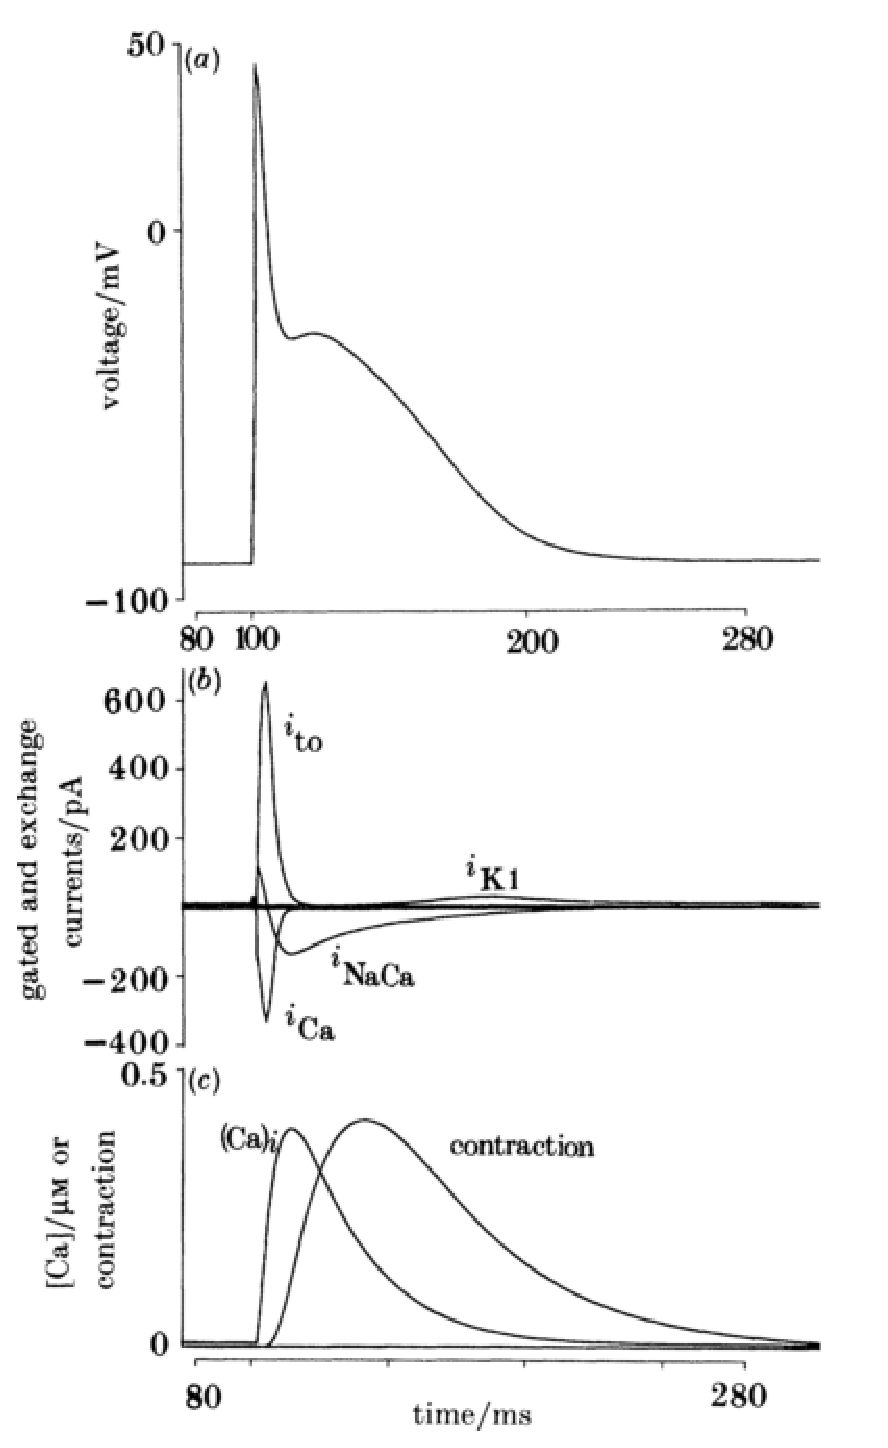
\includegraphics[height=6cm]{./images/Earm1990_current.eps}}
  \caption{Current pulse of 1.3nA applied for 2ms. (A) $V_m$; (B) currents
  carried by $I_\to$, $I_{K1}$ inward rectifier, $I_\NCX$ and $I_\ca$; (C)
  $[\Ca]_i$ transient and force contraction}
  \label{fig:Earm1990_current}
\end{figure}

The calcium current at different value of clamped potential for a duration of
20ms were shown in Fig.\ref{fig:Earm1990_current2}. Here, $I_\na$ and $I_\to$
was set to zero in the simulation. The tail current is the current after the
20ms stimulation. At $V_\clamp=-40$mV and -30mV, the current is small, and
not enough to

\begin{figure}[hbt]
  \centerline{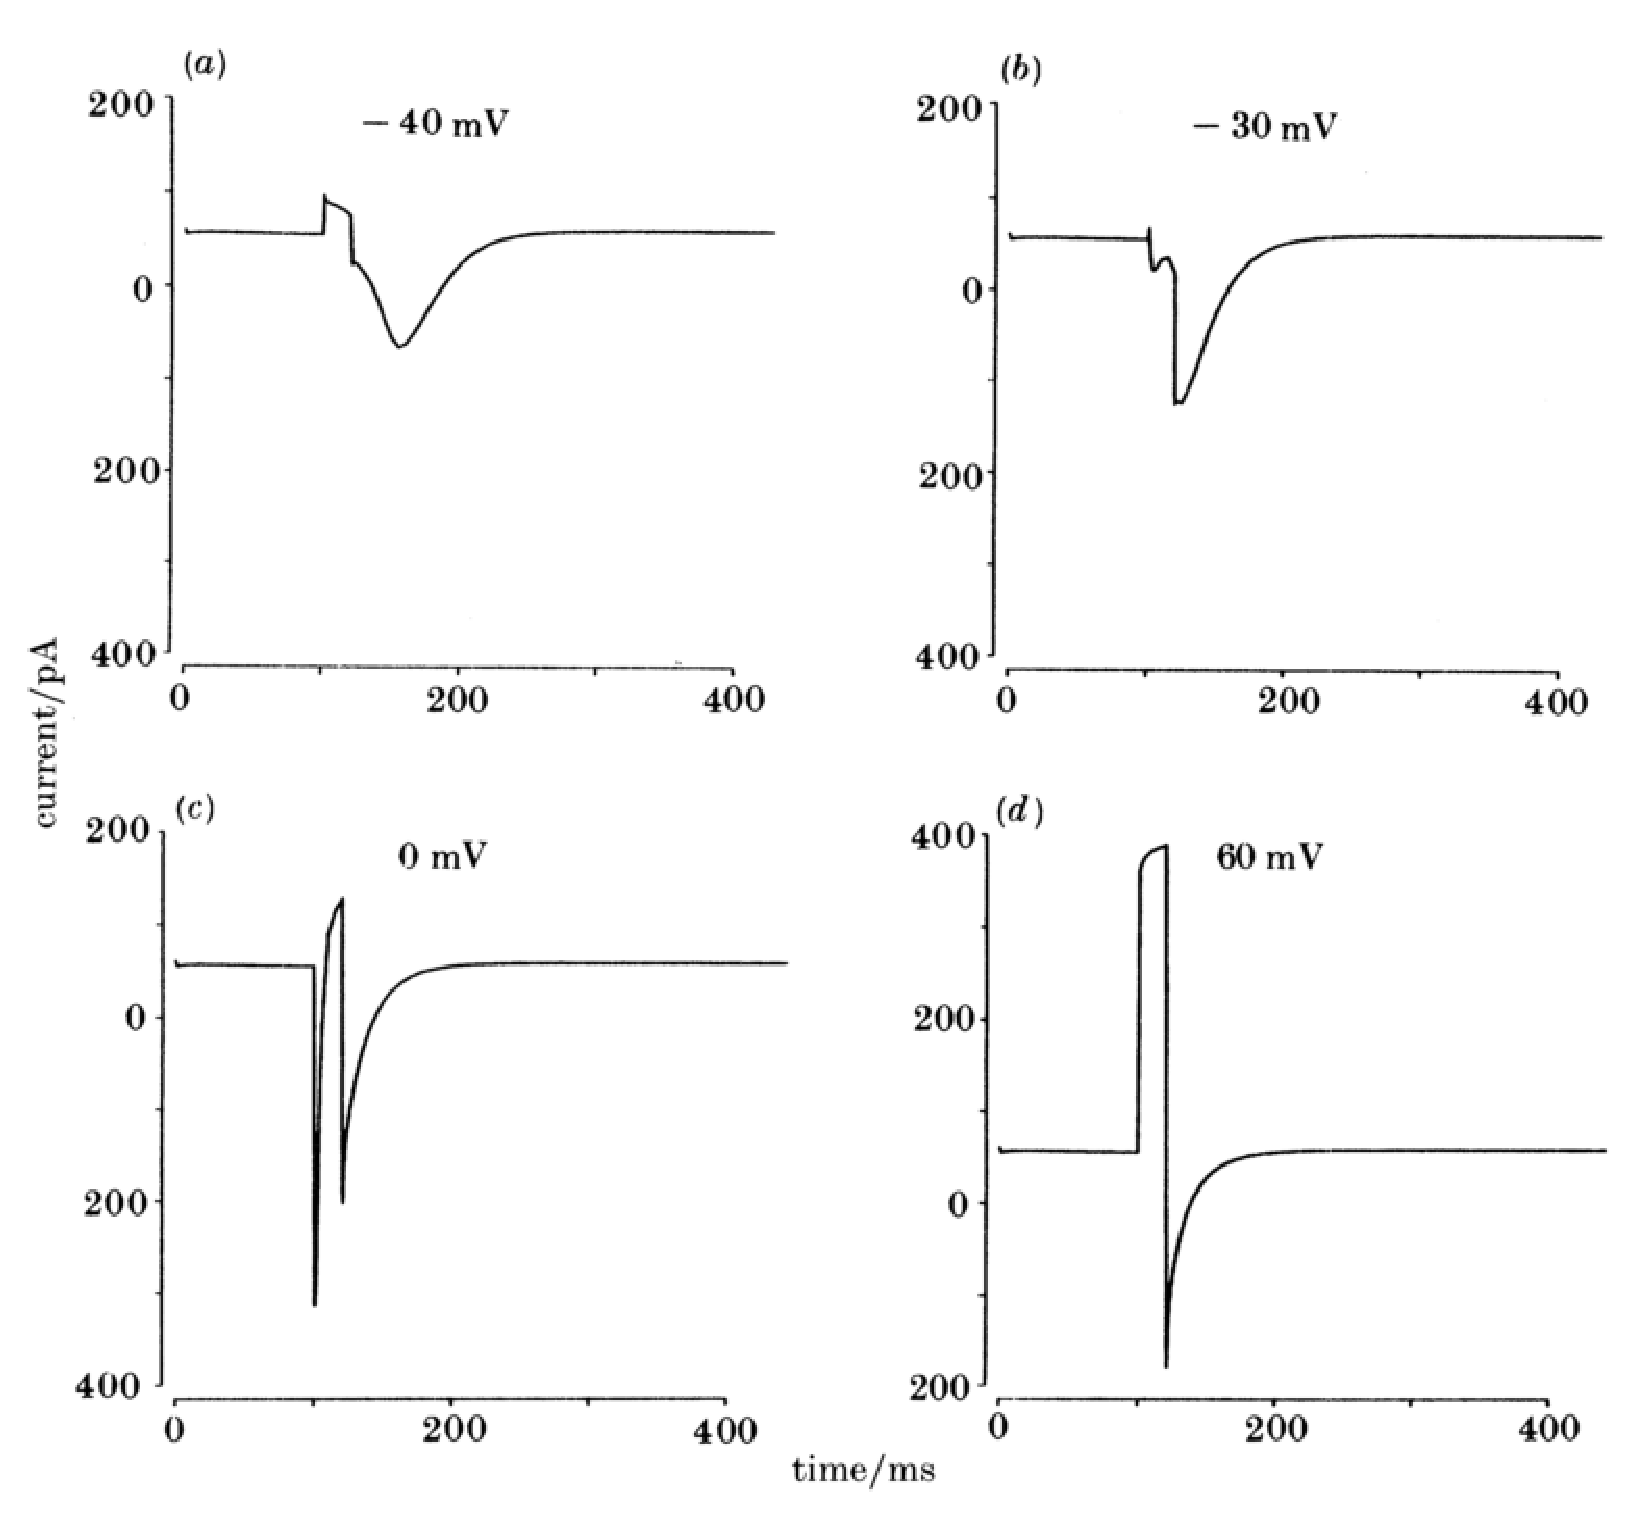
\includegraphics[height=6cm]{./images/Earm1990_Ica.eps}}
  \caption{Voltage-clamp simulated data with 20ms depolarization from -70mV to
  the potential indicated.}
  \label{fig:Earm1990_current2}
\end{figure}

As shown in Fig.4, 20ms voltage clamp of +60mV (from -70mV) is not enough to
trigger $\Ca$ release from SR, giving a small rise in $[\Ca]_i$. At 100ms
stimulation, the calcium entry becomes sufficient to fully trigger calcium
release from SR, after about 50ms. So, we can see an all-or-none behavior in
this model. 

A contradition result obtained by \citep{callewaert1988} using Fura-2 in rat
ventricular cells which show almost zero calcium current. This situation
requires setting $E_{on}=0$. The major difference between the two experimental
settings was 200-400$\muM$ Fura-2 which is a buffer with known $\Ca$-binding
properties \citep{jackson1987}. At high enough concentration of Fura-2, the
buffering properties can be strong enough to reduce the positive feedback
between calcium entry and calcium release, which means more calcium is required
to initiate an full calcium release.


\section[Rasmusson {\it et al.} (1990)]{Rasmusson et al. (frog) (1990)}
\label{sec:rasmusson-et-al}

~\citep{rasmusson1990mme}. 


The model lacks SR, and its role in the dynamics of intracellular
$\ca$. 

\section{Demir {\it et al.} (1994) (SA node) - rabbit}
\label{sec:demir1994_rabbit-atrial}

\citep{Demir1994} developed a single-cell model using data measured at
37$^\circ$C. 


\section{Lindblad et al. (rabit) (1996)}
\label{sec:lindblad-et-al}

~\citep{lindblad1996map} used prominent transient outward ($I_\to$) and rapid
delayed rectifier ($I_\Kr$) currents.

\section{Nygren et al. (human) (1998)}
\label{sec:nygren-et-al}

~\citep{nygren1998mma} used data measured from a atrial appendage tissue
obtained from bypass surgery. 

\section{Courtemanche-Ramirez-Nattel (human) (1998)}
\label{sec:court-ramir-natt}

The model was built based on data measured from atrial appendage
tissue obtained from bypass surgery ~\citep{courtemanche1998imu}.

\section{Ramirez et al. (2000)}
\label{sec:Ramirez_2000}

\citep{ramirez2000}

%%% Local Variables: 
%%% mode: latex
%%% TeX-master: "mainfile"
%%% End: 
